\documentclass{article}

\usepackage[left=2cm,right=2cm, top=2cm, bottom = 2cm]{geometry}
\usepackage{amsfonts}
%%%\usepackage{array}

\usepackage{amsmath}
\usepackage{xcolor}

\usepackage{tikz}
\usepackage{subfigure}

\pagestyle{empty}

\setlength{\tabcolsep}{15pt}
%%%\renewcommand{\arraystretch}{2.5}

%%%\makeatletter
%%%\newcommand{\thickhline}{%
%%%    \noalign {\ifnum 0=`}\fi \hrule height 2pt
%%%    \futurelet \reserved@a \@xhline
%%%}
%%%\newcolumntype{!}{@{\hskip\tabcolsep\vrule width 2pt\hskip\tabcolsep}}
%%%\makeatother

\newcommand{\deriv}[2]{\frac{\mathrm{d}#1}{\mathrm{d}#2}}
\newcommand{\diff}{\;\mathrm{d}}


\usepackage{pgfplots}

\pgfplotsset{compat=1.10}
\usepgfplotslibrary{fillbetween}
\usetikzlibrary{patterns}


\begin{document}

\title{The Fundamental Theorem of Calculus}
\date{}

\maketitle
\thispagestyle{empty}

\Large

\textbf{\underline{Objective: To understand how integration and differentiation relate.}}




\vspace{5mm}


\textbf{Warm-up: Linearity and Adding Integrals:}\bigskip

Recall the definition of the \textbf{integral}:
\[\int_a^b f(x)\diff x =\lim_{n\to\infty}\sum_{k=1}^n f\left(a+\frac{k(b-a)}{n}\right)\frac{b-a}{n}.\]
This gives the area under the graph of $f(x)$ between $x=a$ and $x=b$.

\bigskip


\begin{enumerate}
	\item Thinking in terms of area, write down
		\[\int_a^b f(x)\diff x+\int_b^c f(x)\diff x\]
		as a single integral. Hint: sketch a graph.
	\item We will show that integration is \textbf{linear}---\textit{i.e.}, that
		\[\int_a^b (\alpha f(x)+\beta g(x))\diff x=\alpha\int_a^b f(x)\diff x + \beta\int_a^b g(x)\diff x\]
		for any constants $\alpha$ and $\beta$. (Note: compare with the linearity property of differentiation). To do this:
			\begin{enumerate}
				\item Explain why
					\begin{align*}
						\sum_{k=1}^n \left(\alpha f\left(a+\frac{k(b-a)}{n}\right)+\beta g\left(a+\frac{k(b-a)}{n}\right)\right)\\
						=\alpha\left(\sum_{k=1}^n f\left(a+\frac{k(b-a)}{n}\right)\right) +&\beta\left(\sum_{k=1}^n  g\left(a+\frac{k(b-a)}{n}\right)\right).
					\end{align*}
				\item Why does it follow that integration is linear?
			\end{enumerate}
\end{enumerate}



\clearpage


\textbf{Theory: The Fundamental Theorem of Calculus:}

\bigskip

Differentiation was originally discovered by the French judge and amateur(!) mathematician Pierre de Fermat (of Fermat's method). Integration had kind of been around for millennia---Archimedes of Syracuse showed that the area of a circle is $\pi r^2$ by approximating it with polygons and then considering what happened as the number of sides of the polygon got larger. However, the two notions were unified, and the subject of calculus was born, when the British scientist Isaac Newton and the German philosopher Gottfried Leibniz independently and around the same time discovered the following remarkable result and used it to discover a huge wealth of things concerning differentiation and integration:\bigskip

\noindent\fbox{\parbox{\textwidth}{
	Let $f(x)$ be a continuous function between $x=a$ and $x=b$. Define $F(x)$ for $a\leq x\leq b$ by
	\[F(x)=\int_a^x f(t)\diff t,\]
	so $F(x)$ is the area under the graph of $f$ from $a$ to $x$. Then $F(x)$ is differentiable and
	\[\deriv{F}{x}=f(x).\]
}}\bigskip

In words, the rate-of-change of the area under the graph of $f(x)$ is precisely $f(x)$ itself! Note that here $t$ is simply a ``dummy variable''---since $x$ appears in the limits of the integral, it should not be used as the variable of integration, so we simply substitute another letter.\medskip

The idea of the proof is as follows. The change in $F$ between $x$ and $x+h$ is the area under the graph of $f(x)$ between $x$ and $x+h$, as shown below. So then dividing by $h$ to get the average rate-of-change gives something between $f(x)$ and $f(x+h)$, which tends to $f(x)$ as $h$ tends to 0, by continuity.



\begin{figure}[h]

\subfigure{
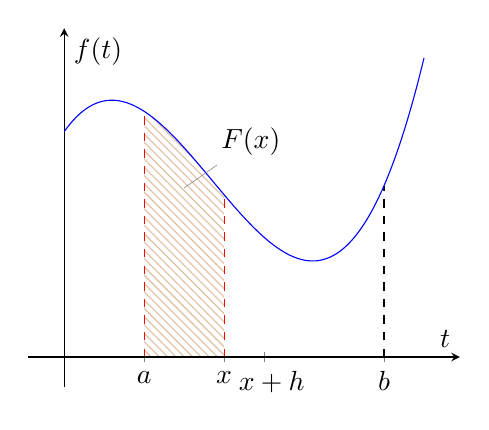
\begin{tikzpicture}[scale=0.8]
	\begin{axis}[axis lines=middle,
		            xlabel=$t$,
		            ylabel=$f(t)$,
	           	 enlargelimits,
           		 ytick=\empty,
		            xtick={1,2,2.5,4},
           	 	xticklabels={$a$,$x$,$\;\;x+h$,$b$}
           	 ]
           	 
           	 \addplot[dashed] coordinates{
           	 	(4,0)
           	 	(4,0.18*64-10)
           	 };
           	 
           	 \addplot [dashed, color=red] coordinates {
           	 	(1,0)
           	 	(1,2.18)
		};
		
		 \addplot [dashed, color=red] coordinates {
           	 	(2,0)
           	 	(2,0.18*8)
		};
		
		\addplot[name path=F,blue,domain={0:4.5},samples=200] {0.18*x^3-x^2+x+2};

		\addplot[name path=G,domain={0:4.5}] {0};

		\addplot[pattern=north west lines, pattern color=brown!50]fill between[of=F and G, soft clip={domain=1:2}];
		\node[coordinate,pin=40:{$F(x)$}] at (axis cs:1.5,1.5){};
	\end{axis}
\end{tikzpicture}
}
\subfigure{
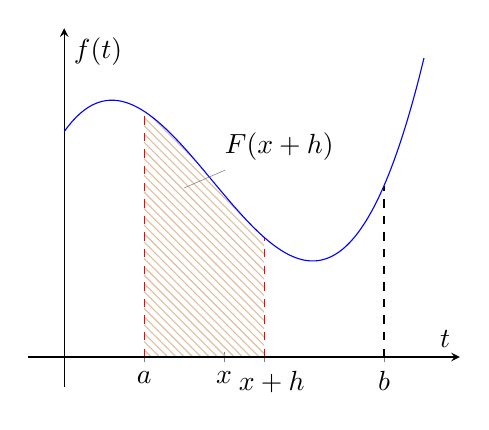
\begin{tikzpicture}[scale=0.8]
	\begin{axis}[axis lines=middle,
			anchor=origin,
		            xlabel=$t$,
		            ylabel=$f(t)$,
	           	 enlargelimits,
           		 ytick=\empty,
		            xtick={1,2,2.5,4},
           	 	xticklabels={$a$,$x$,$\;\;x+h$,$b$}
           	 ]
           	 
           	 \addplot[dashed] coordinates{
           	 	(4,0)
           	 	(4,0.18*64-10)
           	 };
           	  
           	 \addplot [dashed, color=red] coordinates {
           	 	(1,0)
           	 	(1,2.18)
		};
		
		\addplot[dashed,color=red] coordinates {
			(2.5,0)
			(2.5,0.18*2.5^3-2.5^2+4.5)
		};
		
		\addplot[name path=F,blue,domain={0:4.5},samples=200] {0.18*x^3-x^2+x+2};

		\addplot[name path=G,domain={0:4.5}] {0};

		\addplot[pattern=north west lines, pattern color=brown!50]fill between[of=F and G, soft clip={domain=1:2.5}];
		\node[coordinate,pin=30:{$F(x+h)$}] at (axis cs:1.5,1.5){};
	\end{axis}
\end{tikzpicture}
}
\subfigure{
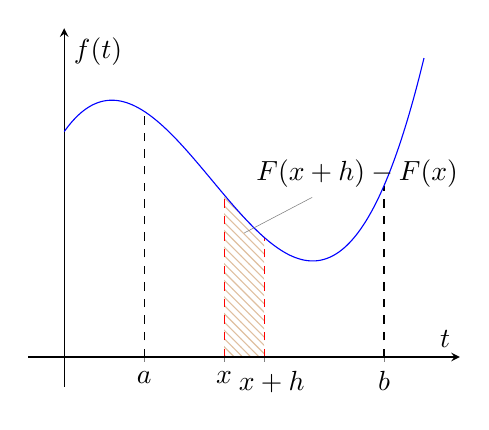
\begin{tikzpicture}[scale=0.8]
	\begin{axis}[axis lines=middle,
		            xlabel=$t$,
		            ylabel=$f(t)$,
	           	 enlargelimits,
           		 ytick=\empty,
		            xtick={1,2,2.5,4},
           	 	xticklabels={$a$,$x$,$\;\;x+h$,$b$}
           	 ]
           	 
           	 \addplot [dashed] coordinates {
           	 	(1,0)
           	 	(1,2.18)
		};
           	 
           	 \addplot[dashed] coordinates{
           	 	(4,0)
           	 	(4,0.18*64-10)
           	 };
           	 
           	  \addplot [dashed, color=red] coordinates {
           	 	(2,0)
           	 	(2,0.18*8)
		};
		
		\addplot[dashed,color=red] coordinates {
			(2.5,0)
			(2.5,0.18*2.5^3-2.5^2+4.5)
		};
		
		\addplot[name path=F,blue,domain={0:4.5},samples=200] {0.18*x^3-x^2+x+2};

		\addplot[name path=G,domain={0:4.5}] {0};

		\addplot[pattern=north west lines, pattern color=brown!50]fill between[of=F and G, soft clip={domain=2:2.5}];
		\node[coordinate,pin=86:{$F(x+h)-F(x)$}] at (axis cs:2.25,1.1){};
	\end{axis}
\end{tikzpicture}
}

\end{figure}

\clearpage

Now we give the details of the proof.\medskip

We need to show that
\[\lim_{h\to 0}\frac{F(x+h)-F(x)}{h}=f(x),\]
since this is the definition of the derivative. But, by definition of $F(x)$, we have
\[F(x+h)-F(x)=\int_a^{x+h}f(t)\diff t - \int_a^x f(t)\diff t.\]
This means the area under the graph of $f(x)$ from $a$ to $x+h$, minus the area from $a$ to $x$---but this is just the area between $x$ and $x+h$:
\[F(x+h)-F(x)=\int_x^{x+h}f(t)\diff t.\]

By the definition of the integral, this is equal to
\[\lim_{n\to \infty}\sum_{k=1}^n f\left(x+\frac{kh}{n}\right)\frac{h}{n},\]
so
\[\frac{F(x+h)-F(x)}{h}=\lim_{n\to \infty}\sum_{k=1}^n f\left(x+\frac{kh}{n}\right)\frac{1}{n},\]
and we want to take the limit of this as $h$ tends to 0.

Now, $f$ is continuous. Recall: this means that for any $x$, as $t\to x$, $f(t)\to f(x)$; so as $n$ tends to infinity and $h$ tends to 0, $x+\frac{kh}{n}$ tends to $x$, and so $f\left(x+\frac{kh}{n}\right)$ tends to $f(x)$. Therefore
\[\lim_{h\to 0}\lim_{n\to \infty}\sum_{k=1}^\infty f\left(x+\frac{kh}{n}\right)\frac{1}{n}=\lim_{n\to \infty}\sum_{k=1}^n f(x)\frac{1}{n}.\]

But now the sum is adding together $n$ copies of $f(x)\frac{1}{n}$, which gives $nf(x)\frac{1}{n}$, which is just $f(x)$. So
\[\deriv{F}{x}=\lim_{h\to 0}\lim_{n\to \infty}\sum_{k=1}^n f\left(x+\frac{kh}{n}\right)\frac{1}{n}=f(x),\]
as we wished to prove.




\clearpage




\textbf{Theory: Antiderivatives:}\bigskip


The Fundamental Theorem is the key that unlocks integration. For differentiation, we saw that it is possible---at least for fairly simple functions---to differentiate directly from the definition; the linearity, chain, and product rules then allow us to differentiate a huge variety of functions quite straightforwardly. Integration, however, is extremely hard to do from the definition for even very simple functions, and it is hard to prove general rules like the product or chain rules to extend the range of functions that can be integrated. The Fundamental Theorem provides a deep link between differentiation and integration that allows us to use our knowledge of derivatives to integrate functions!

This transfer of knowledge from differentiation to integration is facilitated by the notion of an \textbf{antiderivative}; as the name suggests, if $f(x)$ is a function, an antiderivative of $f$ is any function $g(x)$ such that $g'(x)=f(x)$. So another way of stating the Fundamental Theorem is that if $f(x)$ is continuous, then the integral of $f$ is an antiderivative of $f$.

Note that, although a differentiable function has only one derivative (so we can talk about \textit{the} derivative of $f$), a function generally has infinitely many antiderivatives! So we can only ever talk about \textit{an} antiderivative.

However, different antiderivatives of the same function are related in a straightforward way. The reason a function has multiple antiderivatives is that constant terms disappear when differentiating; so if $g(x)$ is an antiderivative of $f(x)$ (\textit{i.e.}, $f$ is the derivative of $g$), then for any constant $c$, $g(x)+c$ is also an antiderivative of $f$. However, this is the only way to get different antiderivatives of a function:\bigskip

\noindent\fbox{\parbox{\textwidth}{
	Let $f(x)$ be a function and $g_1(x)$, $g_2(x)$ be antiderivatives of $f$. Then there is a constant $c$ such that $g_1(x)=g_2(x)+c$.
}}\bigskip

To see why this is true, we use the Mean Value Theorem. Recall that this says that if $h(x)$ is a differentiable function between $a$ and $b$, then there is some $\alpha$ in between $a$ and $b$ such that $h'(\alpha)=\frac{h(b)-h(a)}{b-a}$.

We apply the MVT with $h(x)=g_1(x)-g_2(x)$, (so $h'(x)=g_1'(x)-g_2'(x)$) and \textit{any} two values $a$ and $b$. So there is some $\alpha$ between $a$ and $b$ such that
\[g'_1(\alpha)-g'_2(\alpha)=\frac{h(b)-h(a)}{b-a}.\]
But since $g_1'(x)=f(x)=g_2'(x)$ (as $g_1$ and $g_2$ are antiderivatives of $f$), we must have $g_1'(\alpha)-g_2'(\alpha)=f(\alpha)-f(\alpha)=0$. So for any $a$ and $b$, $h(a)-h(b)=0$, so $h(a)=h(b)$. Therefore $h$ is a constant, so there is some value $c$ such that $h(x)=c$ for all $x$; then $g_1(x)-g_2(x)=c$, so $g_1(x)=g_2(x)+c$, as claimed.



\clearpage
















\textbf{Theory: Evaluating Integrals with Antiderivatives:}\bigskip


The Fundamental Theorem tells us that if we take the integral of a continuous function (to a variable upper limit) and then differentiate, we recover the function we started with. How about going the other way? If $f(x)$ is differentiable, how does the integral of $f'(x)$ relate to $f(x)$? If $f'(x)$ is continuous, then the Fundamental Theorem applies and tells us that
\[\int_a^x f'(t)\diff t\]
is an antiderivative of $f'$ (again, $t$ is a dummy variable here). Since $f$ is certainly an antiderivative of $f'$, and antiderivatives differ only by a constant, we must have
\[\int_a^x f'(t)\diff t = f(x)+c\]
for some constant $c$. This will be true for any $a$ (as long as $f'$ is continuous between $a$ and $x$), but the value of the constant will differ depending on which $a$ we choose; we can, for instance, choose $a$ to be 0. We can use this to evaluate integrals; if we want to integrate $f(x)$ from $a$ to $b$, and we can find an antiderivative $F$ of $f$, then
\begin{align*}
	\int_a^b f(x)\diff x &= \int_0^b f(x)\diff x -\int_0^a f(x)\diff x\\
	&=(F(b)+c)-(F(a)+c)\\
	&=F(b)-F(a).
\end{align*}

\noindent\fbox{\parbox{\textwidth}{
	Let $f(x)$ be a continuous function and $F(x)$ an antiderivative of $f$. Then
	\[\int_a^b f(x)\diff x = F(b)-F(a).\]
}}\bigskip


So to integrate a continuous function from $a$ to $b$, we simply find any antiderivative $F$ and evaluate $F(b)-F(a)$; $F(b)$ is the area up to $b$ plus a constant, $F(a)$ is the area up to $a$ plus the same constant, so $F(b)-F(a)$ is the area between $a$ and $b$ (and the unknown constants cancel out).\medskip



Evaluate
\[\int_2^3 4x^3\diff x.\]




\clearpage





\textbf{Practice:}\bigskip




Since an integral of a continuous function is an antiderivative, we often use the integral notation, but without the limits, as a notation for antiderivatives. We write
\[\int f(x)\diff x = F(x)+c\]
if $F$ is an antiderivative of $f$ (and $c$ is an unknown constant). This is called an \textbf{indefinite integral}, and an integral with limits (to find an area) is called a \textbf{definite integral}, by contrast.\bigskip




\begin{enumerate}
	\item 
		\begin{enumerate}
			\item Differentiate $\frac{2}{3}x^3$.
			\item Hence write down an antiderivative of $2x^2$.
			\item Hence evaluate
				\[\int_0^5 2x^2\diff x.\]
		\end{enumerate}
	\item
		\begin{enumerate}
			\item Differentiate $\sin(2\pi t)$.
			\item Hence find
				\[\int 2\pi \cos(2\pi t)\diff t.\]
			\item Hence evaluate
				\[\int_0^{0.25} 2\pi \cos(2\pi t)\diff t.\]
		\end{enumerate}
	\item
		\begin{enumerate}
			\item Find
				\[\int \frac{1}{2}x^{-1/2}\diff x.\]
			\item Hence evaluate
				\[\int_1^4 \frac{1}{2}x^{-1/2}\diff x.\]
		\end{enumerate}
	\item Evaluate
		\[\int_0^1 e^y \diff y.\]
	\item A particle moves with acceleration $a(t)=6t$, starting with initial velocity $5\mathrm{ms}^{-1}$ at $t=0$.
		\begin{enumerate}
			\item Find the velocity of the particle at time $t$, by evaluating
				\[\int_0^t a(s)\diff s.\]
			\item Find an expression for the distance travelled by the particle at time $t$, by evaluating
				\[\int_0^t v(s)\diff s\]
				(where $s$ is a dummy variable).
		\end{enumerate}
\end{enumerate}








\clearpage













{\bf Key Points to Remember:}

\vspace{5mm}

\begin{enumerate}
	\item Integration is \textbf{linear}: for any integrable functions $f$ and $g$ and any constants $\alpha$ and $\beta$, we have
		\[\int(\alpha f(x)+\beta g(x))\diff x = \alpha\int f(x)\diff x + \beta \int g(x)\diff x.\]
	\item An \textbf{antiderivative} of a function $f(x)$ is any function $F(x)$ such that $F'(x)=f(x)$.
	\item If $F$ and $G$ are both antiderivatives of $f$, then there is a constant $c$ such that $F(x)=G(x)+c$.
	\item The \textbf{Fundamental Theorem of Calculus} says that the integral of a continuous function is an antiderivative:
		\[\deriv{}{t} \int_a^t f(x)\diff x = f(t).\]
	\item We write
		\[\int f(x)\diff x = F(x)+c\]
		if $F$ is an antiderivative of $f$, and call this an \textbf{indefinite integral}.
	\item To evaluate a definite integral of $f(x)$,	find any antiderivative (indefinite integral) $F(x)$ of $f$, and then
		\[\int_a^b f(x)\diff x = F(b)-F(a).\]
	\item The definite integral of the derivative (rate-of-change) of a quantity gives the total amount of change in that quantity between the limits of the integral.
\end{enumerate}









\end{document}